\documentclass[a4paper]{article}

\usepackage[english]{babel}
\usepackage[utf8]{inputenc}
\usepackage{amsmath}
\usepackage{graphicx}
\usepackage[colorinlistoftodos]{todonotes}
\usepackage{hyperref}
\usepackage{listings}
\usepackage[numbers]{natbib}

\usepackage{booktabs} % To thicken table lines



\title{Creating Customer Segments}

\author{Uirá Caiado}

\date{\today}

\begin{document}

\maketitle

\begin{abstract}
As pointed out by \cite{Udacity}, today many companies collect vast amounts of data on their clientele and have a strong desire to understand the meaningful relationships hidden in their customer base. In this project, I will apply unsupervised learning techniques on product spending data collected for consumers of a wholesale distributor in Lisbon, Portugal. My goal is to define how best segment their customers into distinct categories. Afterwards, the segmentation found will be compared with an additional labeling. Lastly, I will suggest ways that the segmentation could assist the wholesale distributor with future service changes.
\end{abstract}

%%%%%%%%%%%%%%%%%%%%%%%%%%%%%%%%%%%%%%%%%%%%%%%%%%%%%%%%%%%%%%%%%%%%%%%%%%%%%%%%%%%%%%%%
%% INTRODUCTION
%%%%%%%%%%%%%%%%%%%%%%%%%%%%%%%%%%%%%%%%%%%%%%%%%%%%%%%%%%%%%%%%%%%%%%%%%%%%%%%%%%%%%%%%

\section{Introduction}
\label{sec:introduction}
In this section, I will give some background about the problem addressed and the goal of the project.

\subsection{Some Background}
As suggested by this article\footnote{Source: \url{http://goo.gl/aEqNpD}}, the current abundance of digital data from many sources — the web, sensors, smartphones and corporate databases — can be mined for discoveries and insights and might lead to smarter, data-driven decision-making in every field.

In this project, I will analyze a dataset containing data on various customers' annual spending amounts of diverse product categories looking for internal structure. One goal of this project is to best describe the variation in the different types of customers that a wholesale distributor interacts with. Doing so would equip the distributor with insight into how to best structure their delivery service to meet the needs of each customer.

Given that there is no previous labeling of each instance in the dataset, I will use unsupervised learning to look for such structure. As explained by \cite{Mitchell}, in this case, there is a set of $N$ observations $(x_1,x_2, ..., x_N )$ of a random vector $X$ that has a joint density $Pr(X)$. The goal is to directly infer the properties of this probability density without the help of a supervisor or teacher providing correct answers or degree-of-error for each observation.

\subsection{Getting Started}
The dataset for this project can be found on the UCI Machine Learning Repository\footnote{Source: \url{https://archive.ics.uci.edu/ml/datasets/Wholesale+customers}}. For the purposes of this project, the features \textit{'Channel'} and \textit{'Region'} will be excluded in the analysis — with focus instead on the six product categories recorded for customers. So, let's start loading the dataset:

% code snipet
\begin{lstlisting}
Wholesale customers dataset has 440 samples with 6 features
each.
\end{lstlisting}

%%%%%%%%%%%%%%%%%%%%%%%%%%%%%%%%%%%%%%%%%%%%%%%%%%%%%%%%%%%%%%%%%%%%%%%%%%%%%%%%%%%%%%%%
%% DATA EXPLORATION
%%%%%%%%%%%%%%%%%%%%%%%%%%%%%%%%%%%%%%%%%%%%%%%%%%%%%%%%%%%%%%%%%%%%%%%%%%%%%%%%%%%%%%%%


\section{Data Exploration}
\label{sec:data_exploration}
In this section, I will begin exploring the data to understand how each feature is related to each others.

\subsection{Basic Statistics}
The six labels explored are continuous and are related to the annual spending on diverse product categories. They are all expressed in in monetary units. The features are:
\begin{itemize}
\item FRESH: fresh products
\item MILK: milk products
\item GROCERY: grocery products
\item FROZEN: frozen products
\item DETERGENTS\_PAPER: detergents and paper products
\item DELICATESSEN: delicatessen products
\end{itemize}

In the Table \ref{tab:basicfacts} below can be observed a statistical description of the dataset:

\begin{table}[ht!]
\centering
\begin{tabular}{l|rrrrrr}
{} &      Fresh &      Milk &   Grocery &    Frozen & Deter. Papr. & Delicatss. \\\hline
count &     440.00 &    440.00 &    440.00 &    440.00 &           440.00 &       440.00 \\
mean  &   12000.30 &   5796.27 &   7951.28 &   3071.93 &          2881.49 &      1524.87 \\
std   &   12647.33 &   7380.38 &   9503.16 &   4854.67 &          4767.85 &      2820.11 \\
min   &       3.00 &     55.00 &      3.00 &     25.00 &             3.00 &         3.00 \\
25\%   &    3127.75 &   1533.00 &   2153.00 &    742.25 &           256.75 &       408.25 \\
50\%   &    8504.00 &   3627.00 &   4755.50 &   1526.00 &           816.50 &       965.50 \\
75\%   &   16933.75 &   7190.25 &  10655.75 &   3554.25 &          3922.00 &      1820.25 \\
max   &  112151.00 &  73498.00 &  92780.00 &  60869.00 &         40827.00 &     47943.00 \\

\end{tabular}
\caption{\label{tab:basicfacts}Statistics About The Dataset.}
\end{table}

\subsection{Selecting Samples}
\label{sec:selecting_samples}
To get a better understanding of the customers and how their data will transform through the analysis, in the Table \ref{tab:sample} I selected a few sample data points and plotted a boxplot in Figure \ref{fig:boxplot} comparing them with the distribution of each feature.

\begin{table}[ht!]
\centering
\begin{tabular}{l|rrrrrr}
{ID} &    Fresh &     Milk &  Grocery &    Frozen & Detergents & Delicatessen \\\hline
1   &  7057.00 &  9810.00 &  9568.00 &   1762.00 &          3293.00 &      1776.00 \\
271 &  2083.00 &  5007.00 &  1563.00 &   1120.00 &           147.00 &      1550.00 \\
413 &  4983.00 &  4859.00 &  6633.00 &  17866.00 &           912.00 &      2435.00 \\

\end{tabular}
\caption{\label{tab:sample}A Sample Of The Original Dataset}
\end{table}

\begin{figure}[ht!]
\centering
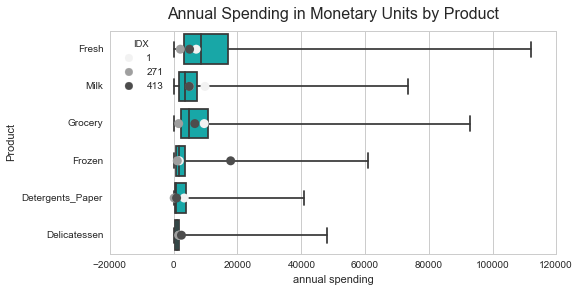
\includegraphics[width=0.85\textwidth]{figures/boxplot_features.png}
\caption{\label{fig:boxplot}Distribution Of The Features}
\end{figure}

Usually data expressed in money, as wealth, expenses, income and so on, are very skewed\footnote{Source: \url{https://en.wikipedia.org/wiki/Skewness}}. As can be seen above, this dataset is not different. The box shows the quartiles of the dataset while the whiskers extend to show the rest of the distribution. There are some customers who spend much more than the median, while the most of them spend around the same level (the data inside the box comprehend 50\% of the dataset).

The data point 271 spent less than 75\% of the other customers (lower quartile) in three product categories: Fresh, Groceries and detergent papers. On the another hand, it spent above the median in products relates to Milk. It could be a small coffee shop, for example. The customer $1$ could be a hotel, as it spent above or expressively above the mean in all product categories, except by Fresh. The last customer selected, 413, has spent at the fourth quartile of the distributions in two products: Frozen, that is well above the third quartile, and delicatessen. It could be a small grocery store.

\subsection{Feature Relevance}
One interesting thought to consider is if one (or more) of the six product categories is actually relevant for understanding customer purchasing. That is to say, is it possible to determine whether customers purchasing some amount of one group of goods will necessarily buy some proportional amount of another category of products? We can make this determination by training a supervised regression learner on a subset of the data with one feature removed and then score how well that model can predict the removed feature.

The table  \ref{tab:r2} shows the $R^{2}$ when attempting to predict different features. The regressions were performed using a Decision Tree\footnote{Source: \url{http://goo.gl/JuLuJH}}. I divided the data between a test and a training set, and then took out one of the features at each iteration to be predicted by all others. Finally, I measured how well those features were relevant to replicate the hold-out column using the coefficient of determination, the $R^{2}$. This coefficient is scored between 0 and 1, with 1 being a perfect fit. A negative $R^2$ implies the model fails to fit the data.

\begin{table}[ht!]
\centering
\begin{tabular}{l|r}
{Predicted} &  Score \\\hline
Fresh            &  -0.77 \\
Milk             &   0.05 \\
Grocery          &   0.74 \\
Frozen           &  -1.41 \\
Detergents\_Paper &   0.56 \\
Delicatessen     &   0.16 \\

\end{tabular}
\caption{\label{tab:r2}The $R^{2}$ when predicting each feature}
\end{table}

As can be seen in the table above, two features, \textit{Grocery} and \textit{Detergents\_Paper}, presented a high $R^2$ score. Around $75$\% and $55$\% of the sample variation in each of the columns used as labels were explained by the other features, respectively. Looking at just this score, I would say that at least the `Grocery` might be unnecessary for identifying customers' spending habits. A good deal of the information on the variability of this feature is contained in others. On the other hand, \textit{Fresh} and \textit{Frozen} presented negative $R^2$, what indicates that the information from them could not be retrieved using other features. In spite of those finds, it is important to point out that low R-squared values\footnote{Source: \url{http://goo.gl/rRAVdJ}} are not inherently bad. This score should always be analyzed in conjunction with other measurements. So, in the next session, I will inspect those relationships visually.


\subsection{Visualize Feature Distributions}

To get a better understanding of the dataset, in the figure \ref{fig:scatter_matrix} I am going to plot a scatter matrix of each of the six product features present in the data. In the main diagonal\footnote{Source: \url{http://www.mathwords.com/m/main_diagonal.htm}} is plotted the distribution of each one. As suggested in section \ref{sec:selecting_samples}, the features are very skewed, apparently showing a Log Normal Distribution\footnote{Source: \url{http://mathworld.wolfram.com/LogNormalDistribution.html}}.

\begin{figure}[ht!]
\centering
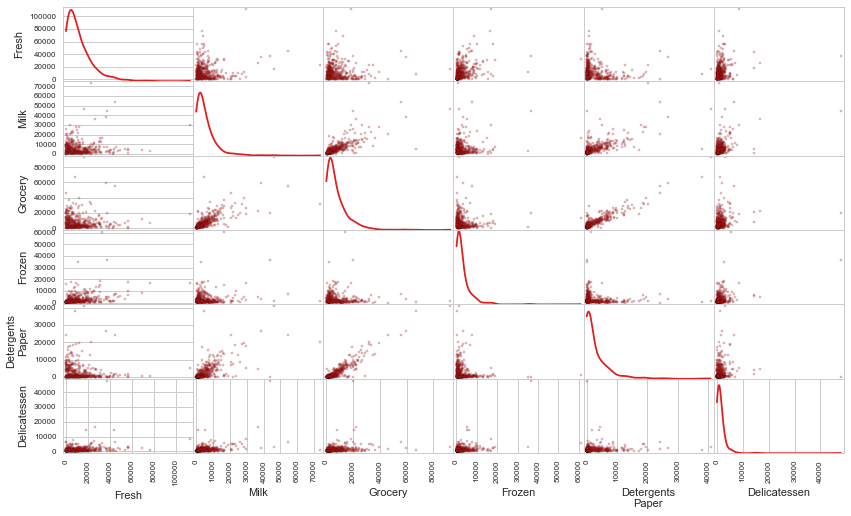
\includegraphics[width=0.75\textwidth]{figures/scatter_matrix.png}
\caption{\label{fig:scatter_matrix}How the Features Correlated}
\end{figure}

As expected, the scatter plot between \textit{Grocery} and \textit{Detergents\_Paper} presented a curious linear relationship. It might suggest that they are complements\footnote{Source: \url{http://www.investopedia.com/terms/c/complement.asp}} to each other. That is, they are consumed in conjunction with other, or they can be complements to a third variable. For example, the \textit{Milk} category seems to be slightly correlated with those features.

The \textit{Fresh} and \textit{Frozen} categories do not correlate to other features at all, as suggested in the last section. However, as the most of the data points are lying in the bottom corner of the charts, it is a little cumbersome to judge the relationships. The Data can be covering some structure. In the next section, I will deal with this characteristic of the dataset.

%%%%%%%%%%%%%%%%%%%%%%%%%%%%%%%%%%%%%%%%%%%%%%%%%%%%%%%%%%%%%%%%%%%%%%%%%%%%%%%%%%%%%%%%
%% DATA PREPROCESSING
%%%%%%%%%%%%%%%%%%%%%%%%%%%%%%%%%%%%%%%%%%%%%%%%%%%%%%%%%%%%%%%%%%%%%%%%%%%%%%%%%%%%%%%%

\section{Data Preprocessing}
\label{sec:data_preprocessing}
In this section, I will preprocess the data to create a better representation of customers by performing a scaling on the data and detecting (and optionally removing) outliers. Preprocessing data is often times a critical step in assuring that results I obtain from my analysis are significant and meaningful.

%%%%%%%%%%%%%%%%%%%%%%%%%%%%%%%%%%%%%%%%%%%%%%%%%%%%%%%%%%%%%%%%%%%%%%%%%%%%%%%%%%%%%%%%
%% FEATURE TRANSFORMATION
%%%%%%%%%%%%%%%%%%%%%%%%%%%%%%%%%%%%%%%%%%%%%%%%%%%%%%%%%%%%%%%%%%%%%%%%%%%%%%%%%%%%%%%%

\section{Feature Transformation}
\label{sec:feature_transformation}
In this section I will use principal component analysis (PCA) to draw conclusions about the underlying structure of the wholesale customer data. Since using PCA on a dataset calculates the dimensions which best maximize variance, we will find which compound combinations of features best describe customers.


%%%%%%%%%%%%%%%%%%%%%%%%%%%%%%%%%%%%%%%%%%%%%%%%%%%%%%%%%%%%%%%%%%%%%%%%%%%%%%%%%%%%%%%%
%% CLUSTERING
%%%%%%%%%%%%%%%%%%%%%%%%%%%%%%%%%%%%%%%%%%%%%%%%%%%%%%%%%%%%%%%%%%%%%%%%%%%%%%%%%%%%%%%%

\section{Clustering}
\label{sec:clustering}
In this section, I will choose to use either a K-Means clustering algorithm or a Gaussian Mixture Model clustering algorithm to identify the various customer segments hidden in the data. I will then recover specific data points from the clusters to understand their significance by transforming them back into their original dimension and scale.


%%%%%%%%%%%%%%%%%%%%%%%%%%%%%%%%%%%%%%%%%%%%%%%%%%%%%%%%%%%%%%%%%%%%%%%%%%%%%%%%%%%%%%%%
%% CONCLUSION
%%%%%%%%%%%%%%%%%%%%%%%%%%%%%%%%%%%%%%%%%%%%%%%%%%%%%%%%%%%%%%%%%%%%%%%%%%%%%%%%%%%%%%%%

\section{Conclusion}
\label{sec:conclusion}
bla

%%%%%%%%%%%%%%%%%%%%%%%%%%%%%%%%%%%%%%%%%%%%%%%%%%%%%%%%%%%%%%%%%%%%%%%%%%%%%%%%%%%%%%%%
%% REFLECTION
%%%%%%%%%%%%%%%%%%%%%%%%%%%%%%%%%%%%%%%%%%%%%%%%%%%%%%%%%%%%%%%%%%%%%%%%%%%%%%%%%%%%%%%%

\section{Reflection}
\label{sec:reflection}
Bla bla bla




\bibliographystyle{plain}
% or try abbrvnat or unsrtnat
\bibliography{bibliography/biblio.bib}
\end{document}
